% -*- encoding: UTF8 -*-
%
%%*****************************************************************************
%---------------------------------------Measurement Results --------------------------------------
%%*****************************************************************************
%
\chapter{Experimental Characterization}
\label{Ch:Measurements}	



%%*****************************************************************************
\section{Fiber Scanner Characterization}
%%*****************************************************************************

\begin{table}[h!]\centering
\begin{tabular}{rccc}
& \textbf{Probe A} & \textbf{Probe B} & \textbf{Probe C} \\ 
\hline
Resonant Frequency [\SI{}{\hertz}] & 765 & 842 & 744 \\ 
Coupling Efficiency & 0.61 & 0.58 & 0.53 \\ 
Backreflectivity [\%]& 0.04 & 0.018 & 0.011 \\ 
Field of View [\SI{}{\milli\meter}]& 1.2 & 1.2 & 1.1 \\ 
\end{tabular} 
\caption{Optomechanical characteristics of three assembled single modality probes.}
    \label{tab:simRes}
\end{table}

Finding operating point\cite{Fertis2006}


%Freq response, coupling of eigendirections
%
%\begin{figure}[h!]\centering \includegraphics[width=10cm,draft]{figures/foo.png}
%      \caption{Pattern of single axis actuation VS Freq}
%      %\label{}
%\end{figure}
%
%
%\begin{figure}[h!]\centering \includegraphics[width=10cm,draft]{figures/foo.png}
%      \caption{Bode plot}
%      %\label{}
%\end{figure}




%%*****************************************************************************

\section{Scanned Imaging}
%%*****************************************************************************

Once that a suitable set of driving parameters has been found for each probe, and the scanner is performing an spiral pattern, the first step to assess the system is to couple light into the probe and measure the intensity of light which is backreflected from the sample. Then, by knowing the backreflected intensity at each point of the spiral it is possible to reconstruct an image of the sample. This imaging technique is thus denominated fiber-optical confocal scanning microscope, whose theory of operation is described in \autoref{ch:theory}.

\subsection{Measurement Setup}
In order to measure the backreflected light intensity it is necessary to send and receive light through the scanning fiber. To achieve this, is it possible to reuse a FD-OCT measurement setup with some modifications. As seen in \autoref{fig:confSetup}, broadband light is coupled from an SLED to a circulator, which forwards it to the probe. After hitting the sample, some of the backscattered light is coupled back into the probe, and is forwarded by the circulator to the photodetector.

\begin{figure}[h!]\centering \includegraphics[width=12cm]{figures/50_Measurements/conf/setup/confSetup.pdf}
      \caption{Measurement setup used for fiber-optical confocal scanning microscopy. Light originating from the SLED is coupled to the probe through the circulator, while the backscattered light from the sample is coupled to the photodetector.}
      \label{fig:confSetup}
\end{figure}

\subsection{Data Processing}
While the probe scans an object with a spiral pattern defined by the driving voltage datapoints $(\mathbf{u_x}[n], \mathbf{u_y}[n])$, the data acquisition system (DAQ) samples a stream of intensities at the photodetector $\mathbf{I}[n]$, as shown in \autoref{fig:confPlotting} a). As these signals are generated and acquired synchronously, we expect that the intensity $\mathbf{I}[i]$ corresponds to a point in object space located at 
$(x, y) = K_\mathrm{mech}(\mathbf{u_x}[i], \mathbf{u_y}[i])$, where $K_\mathrm{mech}$ is a mechanical constant that relates the driving voltage of the piezoelectric scanner to the position of the focus spot assuming a linear behavior. 

\begin{figure}[h!]\centering \includegraphics{figures/50_Measurements/conf/proc/Plotting.pdf}
      \caption{Confocal images}
      \label{fig:confPlotting}
\end{figure}

Now, if all the datapoints $\mathbf{I}_{[n]}$ acquired during a full spiral are plotted as a dot located at the position $K_\mathrm{mech}(\mathbf{u_x}[n], \mathbf{u_y}[n])$, the resultant image would look as in \autoref{fig:confPlotting} b): distorted. Notice how the dot plot defines two overlaid swirled images. This proves that the previous assumption is not valid, and thus the relationship between $(\mathbf{u_x}[i], \mathbf{u_y}[i])$ and $(\mathbf{x}[i], \mathbf{y}[i])$ is neither linear nor simple. This effect is caused by the subtle changes in the dynamic behavior of the fiber scanner at different oscillation amplitudes, and is typical of spiral fiber scanners \cite{Seibel2006}.

There are two general methods to overcome this problem:

The first one involves closed loop operation, where the information of the current position of the scanner is measured inside the probe and fed to the plotting system \cite{Yeoh2014}. 

The open loop alternative, used in this work, assumes that the pattern of the focus spot is constant for a given driving signal. Thus, $(x[i], y[i])$ is measured using a position sensitive device (PSD) after the assembly of the probe and stored as a calibration lookup table. As an example, \autoref{fig:calib} shows the measured values of $(\mathbf{x}[i], \mathbf{y}[i])$ as a point cloud. 
\begin{figure}[h!]\centering \includegraphics[width=6cm]{figures/50_Measurements/conf/proc/samplingDensity.png}
      \caption{Confocal images 21 lp/mm}
      \label{fig:calib}
\end{figure}
Once this calibration step is performed, any further frame is plotted by assigning a position $(\mathbf{x}[i], \mathbf{y}[i])$ to every measured intensity $\mathbf{I}[n]$, as depicted in \autoref{fig:confPlotting} c), which results in the dot plot from \autoref{fig:confPlotting} d). This process is performed in real time.

The dot plots which are obtained from spiral scanners have the inconvenient of non-uniform sampling, as can be seen in \autoref{fig:calib}. Thus, to ease the further processing of the acquired images, it is beneficial to convert the non-uniform dot plot into a cartesian matrix. This can be perform by 2D interpolation.

\subsection{Resolution and Depth of Field Measurement}

\begin{figure}[h!]\centering 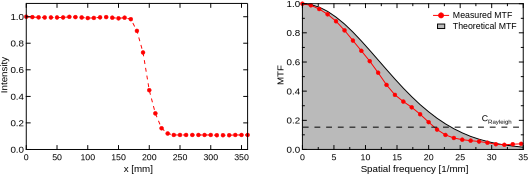
\includegraphics{figures/50_Measurements/conf/res/confResMeas.pdf}
      \caption{Confocal images 21 lp/mm}
      %\label{}
\end{figure}

\begin{figure}[h!]\centering \includegraphics{figures/50_Measurements/conf/res/PSFz.pdf}
      \caption{d}
      %\label{}
\end{figure}

%%*****************************************************************************
\clearpage
\subsection{OCT Imaging}
%%*****************************************************************************
\begin{figure}[h!]\centering \includegraphics{figures/50_Measurements/oct/octSetup.pdf}
      \caption{Measurement setup}
      %\label{}
\end{figure}


Biological samples
\begin{figure}[h!]\centering \includegraphics[width=12cm]{figures/50_Measurements/oct/Measurement_arrangement.png}
      \caption{Biological samples: Vienna B-scan}
      %\label{}
\end{figure}
